\documentclass[fleqn,a4paper,12pt]{article}

%used Packages
\usepackage{standalone}		% Zum Einlesen aus anderen .tex-Files
\usepackage{geometry}		% Zur Bearbeitung des Layouts (Ränder,...)
\usepackage[german]{babel}
\usepackage[utf8]{inputenc}
\usepackage{amsmath}		% Mathematische Symbole
\usepackage{amssymb}     	% Nochmehr mathematische Symbole
\usepackage{dsfont}      	% Schriftsatz fuer Zahlenmengensymbole
%\usepackage{verbatim}   	% erweiterte Verbatim-Umgebung
\usepackage{alltt}       	% Quasi-Verbatim-Umgebung
\usepackage{fancyhdr}    	% Eigene Kopfzeilen
\usepackage{graphicx}    	% Zum Einbinden von Grafiken
							% Einbinden einer eps-Grafik geht so: includegraphics{path}
\usepackage{wrapfig}
\usepackage{lscape}
\usepackage{rotating}
\usepackage{epstopdf}

% Skalierung der Grafiken
\setlength{\unitlength}{1cm}

\frenchspacing               % Kein Extrafreiraum nach Satzzeichen
\setlength{\parindent}{0pt}  % Neue Absaetze nicht einruecken
%\sloppy                     % Schlampige Absatzformatierung
\fussy                       % Penible Absatzformatierung
\linespread{1.5}             % Zeilenabstand


% Seitenraender
\geometry{left=30mm, right=40mm, bottom=30mm}
				% Doc-class, Packageimports, fancy stuff
%%Seitenränder formatieren
\addtolength{\voffset}{-2cm}
\addtolength{\textheight}{0cm}
\addtolength{\hoffset}{0cm}
\addtolength{\textwidth}{2cm}
\addtolength{\headheight}{2cm} % fuer jeden Strichkode einen Zentimeter

% Font fuer Code 39
\font\xlix=wlc39 scaled 1200
\newcommand\barcode[1]{{\xlix@#1@}}

% Name, Matrikelnummer, Barcode
\newcommand\student[2]{
	\mbox{\scriptsize
		\begin{tabular}{@{}l@{}r@{}}
			\multicolumn{2}{@{}r@{}}{\barcode{#2}}\\
			#1&#2\\
		\end{tabular}}}

% Kopfzeile
\pagestyle{fancy}            % Eigene Kopfzeilen verwenden
\lhead{
	\small
	\textsc{Grundlagen der Signalverarbeitung \\
		WS 2017/2018 \\
		\"Ubung (\today)}
	\vfill}
\rhead{
	\begin{tabular}[b]{@{}rr@{}}
		\student{Philipp Badenhoop}{572693} &
		\student{Steven Lange}{568733} \\
		\student{Pascal Jochmann}{575056} &
		\student{Kevin Trogant}{572451}
\end{tabular}}			% Definition der Kopfzeile
%andere Definitionen
\providecommand{\R}{{\mathbb R}}
\providecommand{\N}{{\mathbb N}}
\providecommand{\Z}{{\mathbb Z}}
\providecommand{\Q}{{\mathbb Q}}
\providecommand{\C}{{\mathbb C}}
\providecommand{\F}{\mathcal{F}}
\providecommand{\less}{\setminus}
\providecommand{\inv}{{}^{-1}}
\providecommand{\Land}{\bigwedge}
\providecommand{\Lor}{\bigvee}			% Liste der zusätzlichen Commands und redefines

\begin{document}
	\section*{Übungsaufgabe 19:}
	a) \newline
	\begin{align*}
	\left(\begin{matrix}c_0\\c_1\\c_2\end{matrix}\right) =
	\left(\begin{matrix}
			6.00 & -1.27 & 1.20 & \\
			-1.27 & 3.60 & -0.58 & \\
			1.20 & -0.58 & 3.87 & \\
	\end{matrix}\right)^{-1} \cdot
	\left(\begin{matrix}
			27.00\\
			-20.61\\
			11.64\\
	\end{matrix}\right) \approx
	\left(\begin{matrix}
			3.31\\
			-4.34\\
			1.33\\
	\end{matrix}\right)
	\end{align*}
	$f_{app}(t) = 3.31 \cdot cos(0) + -4.34 \cdot cos(t) + 1.33 \cdot cos(2t) $
	\begin{align*}
			E^2(c) = \sum_{i=0}^5 \left[ f(t_n) - f_{app}(t_n)\right]^2 = 0.58
	\end{align*}

	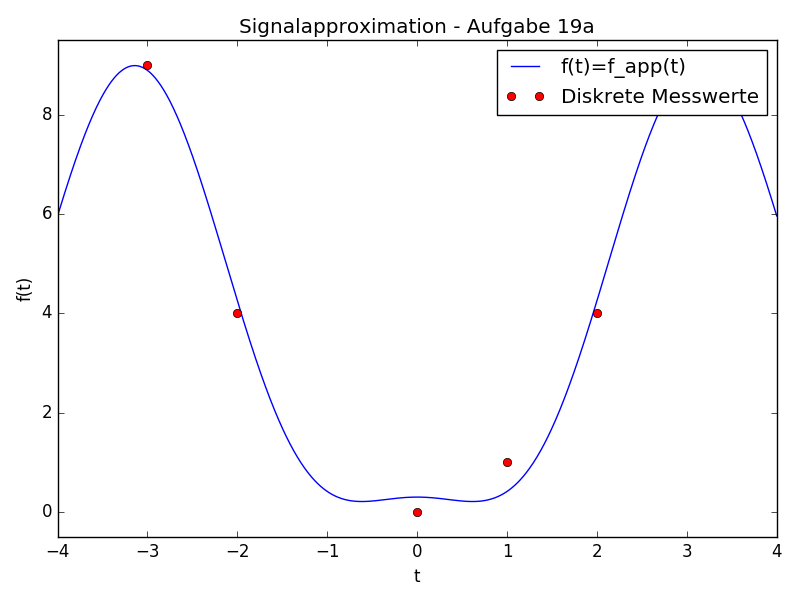
\includegraphics[scale=0.8]{A19a.png}

	b) \newline
	\begin{align*}
	\left(\begin{matrix}c_0\\c_1\\c_2\end{matrix}\right) =
	\left(\begin{matrix}
			6.00 & 0.84 & 0.91 & \\
			0.84 & 2.40 & -0.69 & \\
			0.91 & -0.69 & 2.13 & \\
	\end{matrix}\right)^{-1} \cdot
	\left(\begin{matrix}
			27.00\\
			0.84\\
			0.91\\
	\end{matrix}\right) \approx
	\left(\begin{matrix}
			5.18\\
			-2.18\\
			-2.50\\
	\end{matrix}\right)
	\end{align*}
	$f_{app}(t) = 5.18 \cdot sin(\frac{\pi}{2}) + -2.18 \cdot sin(t) + -2.50 \cdot sin(2t) $
	\begin{align*}
			E^2(c) = \sum_{i=0}^5 \left[ f(t_n) - f_{app}(t_n)\right]^2 = 59.13
	\end{align*}

	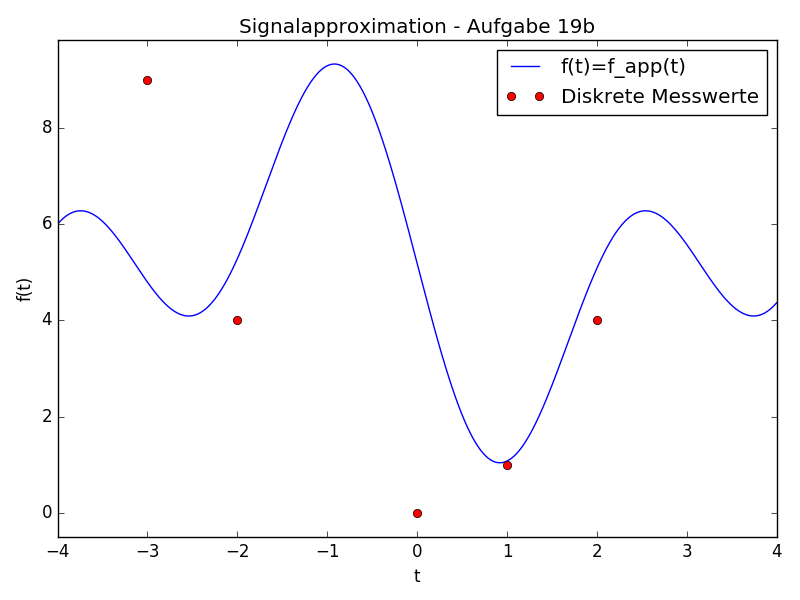
\includegraphics[scale=0.8]{A19b.png}

	c) \newline
	zu a) Punkt (-1,1) hinzugefügt: \newline
	\begin{align*}
	\left(\begin{matrix}c_0\\c_1\\c_2\end{matrix}\right) =
	\left(\begin{matrix}
			7.00 & -0.73 & 0.78 & \\
			-0.73 & 3.89 & -0.81 & \\
			0.78 & -0.81 & 4.04 & \\
	\end{matrix}\right)^{-1} \cdot
	\left(\begin{matrix}
			28.00\\
			-20.07\\
			11.22\\
	\end{matrix}\right) \approx
	\left(\begin{matrix}
			3.41\\
			-4.25\\
			1.27\\
	\end{matrix}\right)
	\end{align*}
	$f_{app}(t) = 3.41 \cdot cos(0) + -4.25 \cdot cos(t) + 1.27 \cdot cos(2t) $\begin{align*}
			E^2(c) = \sum_{i=0}^5 \left[ f(t_n) - f_{app}(t_n)\right]^2 = 0.82
	\end{align*}

	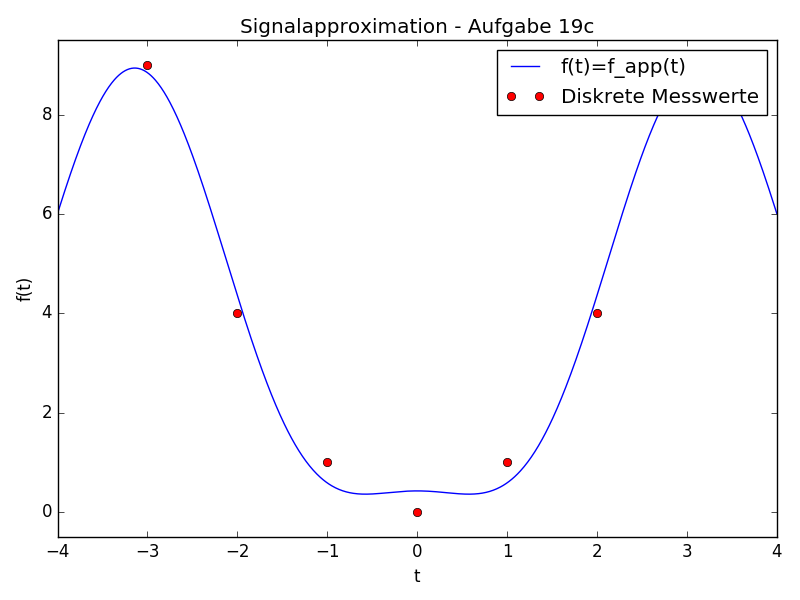
\includegraphics[scale=0.8]{A19c1.png}

	zu b) Punkt (-1,1) hinzugefügt: \newline
	\begin{align*}
	\left(\begin{matrix}c_0\\c_1\\c_2\end{matrix}\right) =
	\left(\begin{matrix}
			7.00 & 0.00 & 0.00 & \\
			0.00 & 3.11 & 0.08 & \\
			0.00 & 0.08 & 2.96 & \\
	\end{matrix}\right)^{-1} \cdot
	\left(\begin{matrix}
			28.00\\
			0.00\\
			0.00\\
	\end{matrix}\right) \approx
	\left(\begin{matrix}
			4.00\\
			0.00\\
			-0.00\\
	\end{matrix}\right)
	\end{align*}
	$f_{app}(t) = 4.00 \cdot sin(\frac{\pi}{2} + 0.00 \cdot sin(t) + -0.00 \cdot sin(2t) $\begin{align*}
			E^2(c) = \sum_{i=0}^5 \left[ f(t_n) - f_{app}(t_n)\right]^2 = 84.00
	\end{align*}

	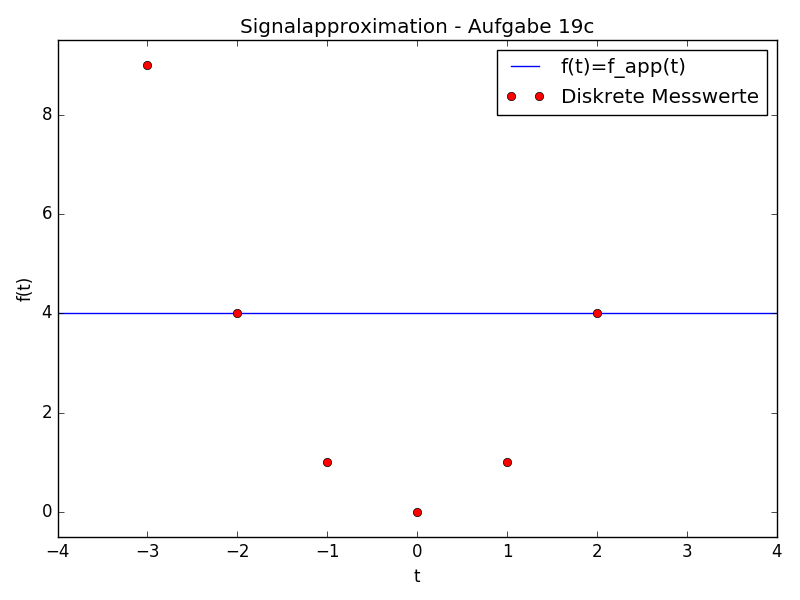
\includegraphics[scale=0.8]{A19c2.png}

	Zusammenfassung: \newline
	Während in a) sich kaum etwas am quadratischen Fehler sowie der Approximationsfunktion ändert, verändert sich die Approximationsfunktion in c) zu einer konstanten Funktion.

\end{document}